\chapter{Validation in Theta}
\section{Overview}
As mention: in the tetha specification.
"Theta is a generic, modular and configurable model checking framework developed at the Critical Systems Research Group of Budapest University of Technology and Economics, aiming to support the design and evaluation of abstraction refinement-based algorithms for the reachability analysis of various formalisms."
The way the Validator for witness 2.0 was implented in Theta is using XCFAs and Product Automaton. Even though 
XCFA's was chosen as formalism for further extensibility in the current version of the validator only the CFA
capabilities where used. For te moment the validator only supports Violation Witnesss. The way the violation
witness verifier works is described in the scheme below.

\begin{figure}[h]
    \centering
    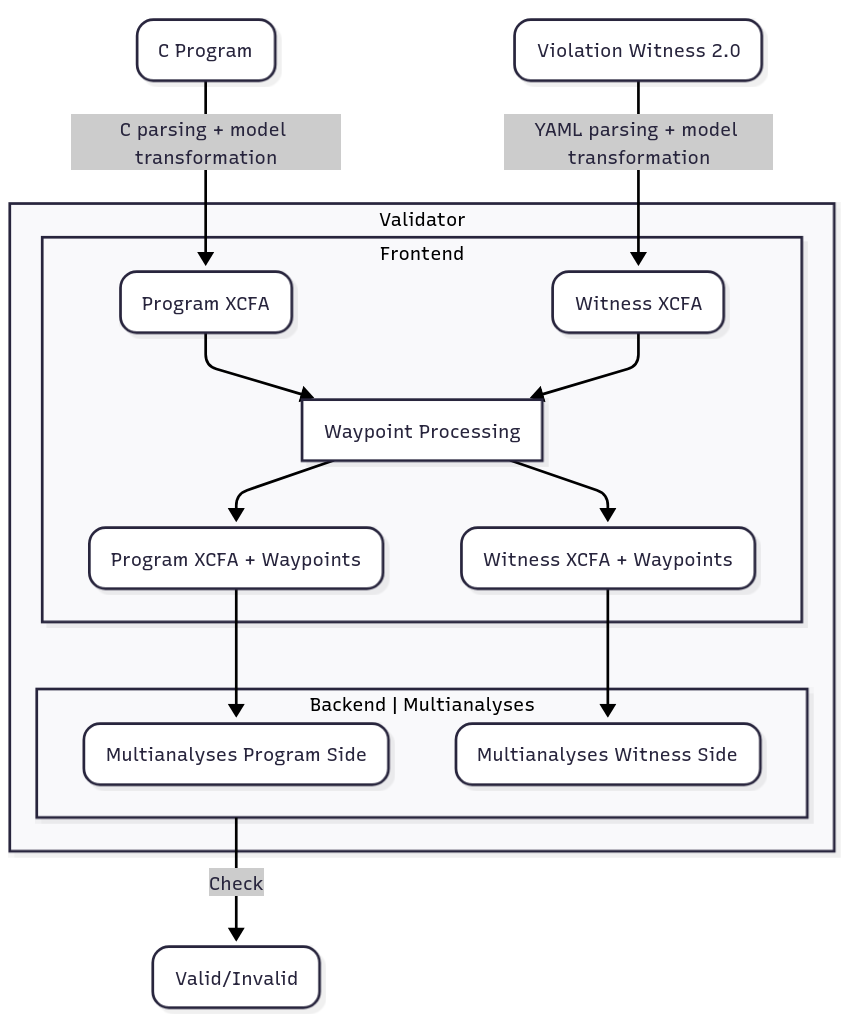
\includegraphics[width=0.8\textwidth]{figures/thetaValidator.png}
    \caption{Validation overview in Theta}
    \label{fig:Validation in Theta}
\end{figure}

% ---
% config:
%       theme: redux
% ---
% flowchart TD
%     cprogram("C Program")
%     witness("Violation Witness 2.0")
    
%     subgraph verifier["Validator"]
%         subgraph frontend["Frontend"]
%             programXCFA("Program XCFA")
%             witnessXCFA("Witness XCFA")
%             subgraph waypointProcessing["Waypoint Processing"]
%             end
%             programXCFAWay("Program XCFA + Waypoints")
%             witnessXCFAWay("Witness XCFA + Waypoints")
%         end
        
%         subgraph backend["Backend | Multianalyses"]
%             multiProgram("Multianalyses Program Side")
%             multiWitness("Multianalyses Witness Side")
%         end
%     end
    
%     output("Valid/Invalid")
    
%     cprogram -->|"C parsing + model transformation"| programXCFA
%     witness -->|"YAML parsing + model transformation"| witnessXCFA
%     programXCFA --> waypointProcessing
%     witnessXCFA --> waypointProcessing
%     waypointProcessing --> programXCFAWay
%     waypointProcessing --> witnessXCFAWay
%     programXCFAWay --> multiProgram
%     witnessXCFAWay --> multiWitness
%     backend -->|"Check"| output


There is no specification (and thus no specific safety property), because for the 
violation witness we are checking the reachability property—whether the error location
in the program and the target location in the witness are reached. The target location
of the witness is modeled as an error state to make the algorithm easy compatible with Multianalyses.

The C program is parsed and transformed into the program XCFA. The witness is parsed as YAML and 
then transformed into the witness XCFA. The violation witness can include waypoints of type avoid. 
In XCFA, a single trap node is created that all avoid waypoints point to. This works because the 
trap node (not connected to any other node) traps the execution of the violation witness, which 
means the error state of this witness cannot be reached.

While transforming the C program from AST to XCFA, much of the AST node data is added as metadata 
to the XCFA locations and edges. This metadata is used to ensure that the waypoints of the witness 
point to the correct places in the program XCFA. The pointing and correlation between the XCFAs are 
done using a global variable waypoint, which is assigned in the program XCFA and assumed in the 
witness XCFA.

From each XCFA, a Multianalysis side is created. Then the sides are combined to form the Multianalysis. 
Because of how the waypoint variable is handled, the Multianalysis is straightforward: each side 
is moved in sequence, starting from the program XCFA, until error states are reached in both XCFAs.

If both error states are reached, the witness is considered valid; otherwise, it is considered invalid.

\section{Example}
To clarify how the validator works, we provide a detailed example of its execution.
The program and the its cooresponding witness we will examine is as follows:

\begin{lstlisting}[style=c,caption=C Program,label=lst:code]
void reach_error(){}
extern unsigned char __VERIFIER_nondet_uchar(void);
int main() {
  unsigned char n = __VERIFIER_nondet_uchar();
  if (n == 0) return 0;
  
  unsigned char v = 0;
  unsigned char s = 0;
  unsigned int i = 0;
  
  while (i < n) {
    v = __VERIFIER_nondet_uchar();
    s += v;
    ++i;
  }
  
  if (s < v) { reach_error(); return 1; }
  if (s > 65025) { reach_error(); return 1; }
  
  return 0;
}
\end{lstlisting}

\begin{lstlisting}[style=yaml, language=C,caption=Violation Witness]
- entry_type: "violation_sequence"
metadata:
    format_version: "2.0"
    uuid: "4412af70-389a-475e-849c-e57e5b92019e"
    creation_time: "2023-09-28T14:42:30+02:00"
    producer:
        name: "CPAchecker"
        version: "2.2.1-svn"
        configuration: "svcomp23"
    task:
        input_files:
        - "unsafe-program-example.c"
        input_file_hashes:
        "unsafe-program-example.c": "788d7646eac82f609530b21c31663b77db1405e2b5e4d86a794d2b2e4367fb8a"
        specification: "G ! call(reach_error())"
        data_model: "ILP32"
        language: "C"
content:
- segment:
    - waypoint:
        type: "branching"
        action: "follow"
        constraint:
            value: "false"
        location:
            file_name: "unsafe-program-example.c"
            line: 11
            column: 3
- segment:
    - waypoint:
        type: "assumption"
        action: "follow"
        constraint:
            value: "v == 0"
            format: "c_expression"
        location:
            file_name: "unsafe-program-example.c"
            line: 15
            column: 3
            function: "main"
- segment:
    - waypoint:
        type: "assumption"
        action: "follow"
        constraint:
            value: "s == 0"
            format: "c_expression"
        location:
            file_name: "unsafe-program-example.c"
            line: 16
            column: 3
            function: "main"
- segment:
    - waypoint:
        type: "branching"
        action: "follow"
        constraint:
            value: "true"
        location:
            file_name: "unsafe-program-example.c"
            line: 17
            column: 3
            function: "main"
- segment:
    - waypoint:
        type: "target"
        action: "follow"
        location:
            file_name: "unsafe-program-example.c"
            line: 23
            column: 5
            function: "main"
\end{lstlisting}

Unfortunetily, the XCFA of the program is quite complex and holds quite large amounts of information.
Therefore here we are going to work with a simplied version of the program XCFA.

Take ti from digrapth put it on mermaid and simplify bothe winesses

Here is the witness:

Here are the witness after the waypoint are mached
Here show both XCFAs and show the code in between pointing wher the witnesses are pointing

Explain hwo the the XCFAs would be executed one after each other.

\section{Theta's Validation Capabilities Compared to Other Verification Tools}
